\documentclass[12pt,twoside]{article}

\textwidth 17cm \textheight 25cm \evensidemargin 0cm
\oddsidemargin 0cm \topmargin -2cm
\parindent 0pt
%\parskip \bigskipamount

\usepackage{graphicx}
\usepackage[dutch]{babel}
\usepackage{amssymb,amsthm,amsmath}
%\usepackage{dot2texi}
\usepackage[utf8]{inputenc}
\usepackage{nopageno}
\usepackage{pdfpages}
\usepackage{enumerate}
\usepackage{caption}
\usepackage{wrapfig}
\usepackage{pgf,tikz,pgfplots}
\pgfplotsset{compat=1.15}
\usepackage{color}
\usetikzlibrary{arrows}
\usetikzlibrary{patterns}
\usepackage{fancyhdr}
\pagestyle{fancy}
\usepackage[version=3]{mhchem}
\usepackage{multicol}
\usepackage{fix-cm}
\usepackage{setspace}
\usepackage{mhchem}
\usepackage{xhfill}
\usepackage{parskip}
\usepackage{cancel}
\usepackage{mdframed}
\usepackage{url}
\usepackage{mathtools}
\usepackage{changepage}

\newcommand{\todo}[1]{{\color{red} TODO: #1}}

\newcommand{\degree}{\ensuremath{^\circ}}
\newcommand\rad{\qopname\relax o{\mathrm{rad}}}

\newcommand\ggd{\qopname\relax o{\mathrm{ggd}}}

\pgfmathdeclarefunction{gauss}{2}{%
  \pgfmathparse{1/(#2*sqrt(2*pi))*exp(-((x-#1)^2)/(2*#2^2))}%
}

\def\LRA{\Leftrightarrow}

\newcommand{\zrmbox}{\framebox{\phantom{EXE}}\phantom{X}}
\newcommand{\zrm}[1]{\framebox{#1}}

% environment oefening:
% houdt een teller bij die de oefeningen nummert, probeert ook de oefening op één pagina te houden
\newcounter{noefening}
\setcounter{noefening}{0}
\newenvironment{oefening}
{
  \stepcounter{noefening}
  \pagebreak[0]
  \begin{minipage}{\textwidth}
  \vspace*{0.7cm}{\large\bf Oefening \arabic{noefening}}
}{%
  \end{minipage}
}

\usepackage{calc}

% vraag
\reversemarginpar
\newcounter{punten}
\setcounter{punten}{0}
\newcounter{nvraag}
\setcounter{nvraag}{1}
\newlength{\puntwidth}
\newlength{\boxwidth}
\newcommand{\vraag}[1]{
\settowidth{\puntwidth}{\Large{#1}}
\setlength{\boxwidth}{1.5cm}
\addtolength{\boxwidth}{-\puntwidth}
{\large\bf Vraag \arabic{nvraag} \addtocounter{nvraag}{1}}\vspace*{-0.5cm}
{\marginpar{\color{lightgray}\fbox{\parbox{1.5cm}{\vspace*{1cm}\hspace*{\boxwidth}{\Large{#1}}}}}
\vspace*{0.5cm}}
\addtocounter{punten}{#1}}

% arulefill
\def\arulefill{\leavevmode{\xrfill[-5pt]{0.3pt}[lightgray]\endgraf}\vspace*{0.2cm}}

% \arules{n}
\newcommand{\arules}[1]{
\color{lightgray}
%\vspace*{0.05cm}
\foreach \n in {1,...,#1}{
  \vspace*{0.75cm}
  \hrule height 0.3pt\hfill
}\color{black}\vspace*{0.2cm}}

% \arule{x}
\newcommand{\arule}[1]{
\color{lightgray}{\raisebox{-0.1cm}{\rule[-0.05cm]{#1}{0.3pt}}}\color{black}
}

% \abox{y}
\newcommand{\abox}[1]{
\fbox{
\begin{minipage}{\textwidth- 4\fboxsep}
\hspace*{\textwidth}\vspace{#1}
\end{minipage}
}
}

\newcommand{\ruitjes}[1]{
\definecolor{cqcqcq}{rgb}{0.85,0.85,0.85}
\hspace*{-2.5cm}
\begin{tikzpicture}[scale=1.04,line cap=round,line join=round,>=triangle 45,x=1.0cm,y=1.0cm]
\draw [color=cqcqcq, xstep=0.5cm, ystep=0.5cm] (0,-#1) grid (20.5,0);
\end{tikzpicture}
}


\newcommand{\assenstelsel}[5][1]{
\definecolor{cqcqcq}{rgb}{0.65,0.65,0.65}
\begin{tikzpicture}[line cap=round,line join=round,>=triangle 45,x=#1cm,y=#1cm]
\draw [color=cqcqcq,dash pattern=on 1pt off 1pt, xstep=1.0cm,ystep=1.0cm] (#2,#4) grid (#3,#5);
\draw[->,color=black] (#2,0) -- (#3,0);
%\draw[shift={(1,0)},color=black] (0pt,2pt) -- (0pt,-2pt) node[below] {\footnotesize $1$};
%\draw[color=black] (#3.25,0.07) node [anchor=south west] {$x$};
\draw[->,color=black] (0,#4) -- (0,#5);
%\draw[shift={(0,1)},color=black] (2pt,0pt) -- (-2pt,0pt) node[left] {\footnotesize $1$};
\draw[color=black] (0.09,#5.25) node [anchor=west] {\phantom{$y$}};
%\draw[color=black] (0pt,-10pt) node[right] {\footnotesize $0$};
\end{tikzpicture}
}

\newcommand{\getallenas}[3][1]{
\definecolor{cqcqcq}{rgb}{0.65,0.65,0.65}
\begin{tikzpicture}[scale=#1,line cap=round,line join=round,>=triangle 45,x=1.0cm,y=1.0cm]
\draw [color=cqcqcq,dash pattern=on 1pt off 1pt, xstep=1.0cm,ystep=1.0cm] (#2,-0.2) grid (#3,0.2);
\draw[->,color=black] (#2.25,0) -- (#3.5,0);
\draw[shift={(0,0)},color=black] (0pt,2pt) -- (0pt,-2pt) node[below] {\footnotesize $0$};
\draw[shift={(1,0)},color=black] (0pt,2pt) -- (0pt,-2pt) node[below] {\footnotesize $1$};
\draw[color=black] (#3.25,0.07) node [anchor=south west] {$\mathbb{R}$};
\end{tikzpicture}
}

\newcommand{\visgraad}[1]{\begin{tabular}{p{0.5cm}|p{#1}}&\\\hline\\\end{tabular}}

\newcommand{\tekenschema}[2]{\begin{tabular}{p{0.5cm}|p{#1}}&\\\hline\\[#2]\end{tabular}}

% schema van Horner
\newcommand{\schemahorner}{
\begin{tabular}{p{0.5cm}|p{7cm}}
&\\[1.5cm]
\hline\\
\end{tabular}}

% geef tabular iets meer ruimte
\setlength{\tabcolsep}{14pt}
\renewcommand{\arraystretch}{1.5}

\newcommand{\toets}[3]{
\thispagestyle{plain}
\vspace*{-2.5cm}
\begin{tikzpicture}[remember picture, overlay]
    \node [shift={(15.25 cm,-1.6cm)}] {%
        \includegraphics[width=1.8cm]{/home/ppareit/kaa1415/logokaavelgem.png}%
    };%
\end{tikzpicture}

\begin{tabular}{|llc|c|}
\hline
\vspace*{-0.5cm}
&&&\\
Naam & \arule{4cm} & {\Large\bf KA AVELGEM} & \\
\vspace*{-0.75cm}
&&&\\
Klas & \arule{4cm} & {\Large\bf 20...-...-...} & \\
\hline
\vspace*{-0.75cm}
&&&\\
Toets & {\bf #2} & {\large\bf #1} & Beoordeling\\
\vspace*{-0.75cm}
&&&\\
Onderwerp & \multicolumn{2}{l|}{\bf #3} &\\
\hline
\end{tabular}
}

\newcommand{\oefeningen}[1]{

\fancyhead[LE, RO]{\vspace{0.5cm} #1}
%\thispagestyle{plain}

{\bf \Large \centering Oefeningen: #1}

}

\raggedbottom

\newcommand\vl{\qopname\relax o{\mathrm{vl}}}

\newcommand\dom{\qopname\relax o{\mathrm{dom}}}
\newcommand\ber{\qopname\relax o{\mathrm{ber}}}

\newcommand\mC{\qopname\relax o{\mathrm{mC}}}
\newcommand\uC{\qopname\relax o{\mathrm{{\mu}C}}}
\newcommand\C{\qopname\relax o{\mathrm{C}}}

\newcommand\W{\qopname\relax o{\mathrm{W}}}
\newcommand\kW{\qopname\relax o{\mathrm{kW}}}
\newcommand\kWh{\qopname\relax o{\mathrm{kWh}}}


\newcommand\V{\qopname\relax o{\mathrm{V}}}
\newcommand\ohm{\qopname\relax o{\mathrm{\Omega}}}
\newcommand\kohm{\qopname\relax o{\mathrm{k\Omega}}}


\newcommand\N{\qopname\relax o{\mathrm{N}}}

\newcommand\Nperkg{\qopname\relax o{\mathrm{N/kg}}}

\newcommand\Nperm{\qopname\relax o{\mathrm{N/m}}}

\newcommand\gpermol{\qopname\relax o{\mathrm{g/mol}}}


\newcommand\kgperm{\qopname\relax o{\mathrm{kg/m}}}
\newcommand\kgperdm{\qopname\relax o{\mathrm{kg/dm}}}
\newcommand\gpercm{\qopname\relax o{\mathrm{g/cm}}}
\newcommand\gperml{\qopname\relax o{\mathrm{g/ml}}}


\newcommand{\mA}{\;\mbox{mA}}
\newcommand{\A}{\;\mbox{A}}
\newcommand{\MA}{\;\mbox{MA}}

\newcommand{\us}{\;\mu\mbox{s}}
\newcommand\s{\qopname\relax o{\mathrm{s}}}

\newcommand\h{\qopname\relax o{\mathrm{h}}}

\newcommand{\kmperh}{\;\mbox{km/h}}
\newcommand{\mpers}{\;\mbox{m/s}}
\newcommand{\kmpermin}{\;\mbox{km/min}}
\newcommand{\kmpers}{\;\mbox{km/s}}

\newcommand{\mph}{\;\mbox{mph}}

\newcommand{\Hz}{\;\mbox{Hz}}

\newcommand\Gm{\qopname\relax o{\mathrm{Gm}}}
\newcommand\Mm{\qopname\relax o{\mathrm{Mm}}}
\newcommand\km{\qopname\relax o{\mathrm{km}}}
\newcommand\hm{\qopname\relax o{\mathrm{hm}}}
\newcommand\dam{\qopname\relax o{\mathrm{dam}}}
\newcommand\m{\qopname\relax o{\mathrm{m}}}
\newcommand\dm{\qopname\relax o{\mathrm{dm}}}
\newcommand\cm{\qopname\relax o{\mathrm{cm}}}
\newcommand\mm{\qopname\relax o{\mathrm{mm}}}
\newcommand\um{\qopname\relax o{\mathrm{{\mu}m}}}
\newcommand\nm{\qopname\relax o{\mathrm{nm}}}


\newcommand\Gg{\qopname\relax o{\mathrm{Gg}}}
\newcommand\Mg{\qopname\relax o{\mathrm{Mg}}}
\newcommand\kg{\qopname\relax o{\mathrm{kg}}}
\newcommand\hg{\qopname\relax o{\mathrm{hg}}}
\renewcommand\dag{\qopname\relax o{\mathrm{dag}}}
\newcommand\g{\qopname\relax o{\mathrm{g}}}
\newcommand\dg{\qopname\relax o{\mathrm{dg}}}
\newcommand\cg{\qopname\relax o{\mathrm{cg}}}
\newcommand\mg{\qopname\relax o{\mathrm{mg}}}
\newcommand\ug{\qopname\relax o{\mathrm{{\mu}g}}}
\renewcommand\ng{\qopname\relax o{\mathrm{ng}}}

\newcommand\ton{\qopname\relax o{\mathrm{ton}}}

\newcommand\Gl{\qopname\relax o{\mathrm{Gl}}}
\newcommand\Ml{\qopname\relax o{\mathrm{Ml}}}
\newcommand\kl{\qopname\relax o{\mathrm{kl}}}
\newcommand\hl{\qopname\relax o{\mathrm{hl}}}
\newcommand\dal{\qopname\relax o{\mathrm{dal}}}
\renewcommand\l{\qopname\relax o{\mathrm{l}}}
\newcommand\dl{\qopname\relax o{\mathrm{dl}}}
\newcommand\cl{\qopname\relax o{\mathrm{cl}}}
\newcommand\ml{\qopname\relax o{\mathrm{ml}}}
\newcommand\ul{\qopname\relax o{\mathrm{{\mu}l}}}
\newcommand\nl{\qopname\relax o{\mathrm{nl}}}

\newcommand\MJ{\qopname\relax o{\mathrm{MJ}}}
\newcommand\kJ{\qopname\relax o{\mathrm{kJ}}}
\newcommand\J{\qopname\relax o{\mathrm{J}}}

\newcommand\T{\qopname\relax o{\mathrm{T}}}
\newcommand\uT{\qopname\relax o{\mathrm{{\mu}T}}}

\newcommand\grC{\qopname\relax o{\mathrm{{\degree}C}}}

\newcommand\K{\qopname\relax o{\mathrm{K}}}
\newcommand\calperK{\qopname\relax o{\mathrm{cal/K}}}

\newcommand\hPa{\qopname\relax o{\mathrm{hPa}}}
\newcommand\Pa{\qopname\relax o{\mathrm{Pa}}}

\newcommand\dB{\qopname\relax o{\mathrm{dB}}}

\newcommand\Var{\qopname\relax o{\mathrm{Var}}}

\newcommand{\EE}[1]{\cdot 10^{#1}}

\onehalfspacing

%\setlength{\headsep}{0cm}

\newenvironment{exlist}[1] %
{ \begin{multicols}{#1}
  \begin{enumerate}[(a)]
    \setlength{\itemsep}{0.5em} }
{ \end{enumerate}
  \end{multicols} }




\begin{document}

\thispagestyle{empty}
\begin{center}
  \begin{mdframed}
    \centering
    \fontsize{40}{60}\selectfont Matrices en Stelsels
  \end{mdframed}
  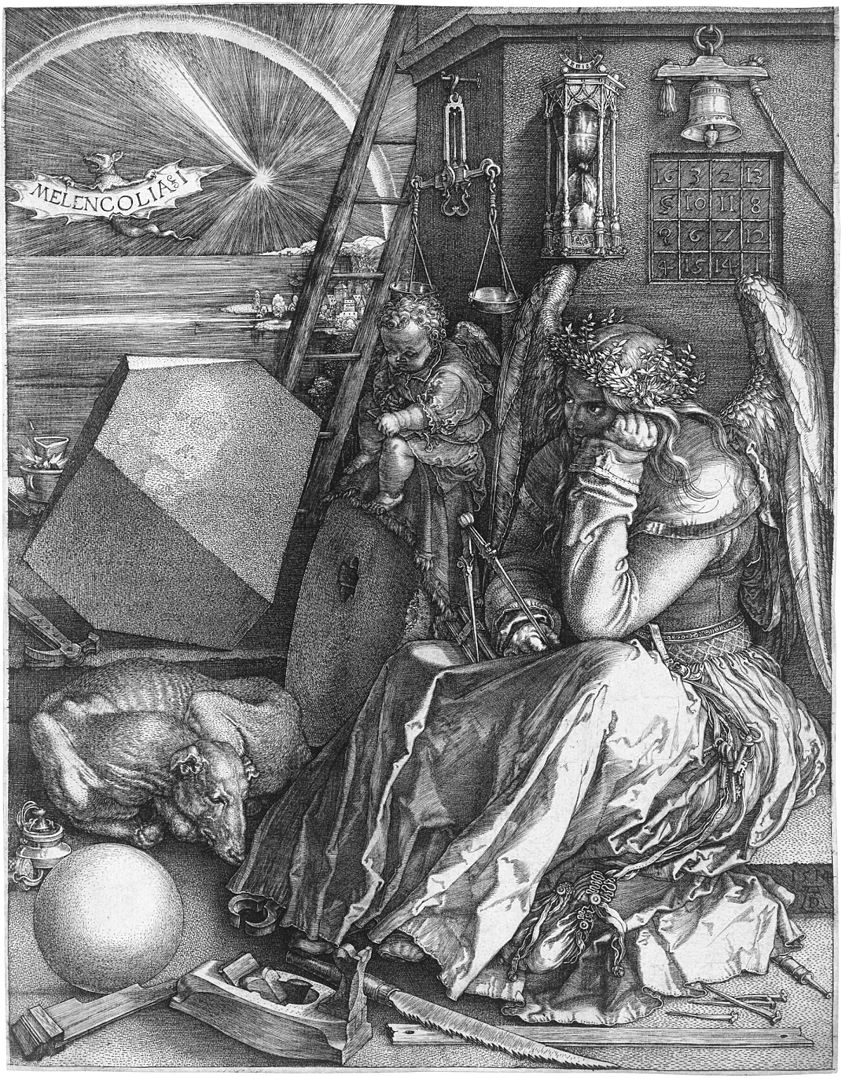
\includegraphics[width=7cm]{magicsquare}
  %\vfill
\end{center}

\subsection*{Doelstellingen}
\begin{singlespacing}
  Je \hfill  {\scriptsize(LP2006-059, LI1.9, ET32,14,31)}
  \begin{itemize}
    \itemsep-0.2em
  \item kent de definitie van een matrix
  \item kent een rijmatrix, een kolommatrix, een vierkante matrix, een driehoeksmatrix, een diagonaalmatrix, de eenheidsmatrix, de nulmatrix
  \item kan matrices optellen, vermenigvuldigen met een reëel getal en vermenigvuldigen
  \item kan matrices transponeren
  \item kan met behulp van ICT vraagstukken oplossen die aanleiding geven tot een migratiematrix of een Lesliematrix
  \item kan van een gegeven stelsel van vergelijkingen van de eerste graad de bijhorende coëfficiëntenmatrix en verhoogde matrix bepalen
  \item kan elementaire rijoperaties toepassen die de gelijkwaardigheid van de overeenstemmende stelsels van vergelijkingen van de eerste graad bewaren
  \item kan de oplossingsmethode van Gauss-Jordan toepassen
  \item kan vraagstukken oplossen die aanleiding geven tot een stelsel van vergelijkingen van de eerste graad
  \end{itemize}
\end{singlespacing}

\thispagestyle{empty}
\clearpage

\tableofcontents
\thispagestyle{empty}
\clearpage

\pagenumbering{arabic}

\pagestyle{fancy}
\fancyhead[RO,LE]{Matrices en Stelsels}
\fancyhead[RE,LO]{}

\section{Definitie}

\subsection{Voorbeeld}

De tabel
$$\begin{pmatrix}3 & \sqrt{2} & -5\\ \pi & 0 & \dfrac{1}{2}\end{pmatrix}$$
noemen we een matrix met 2 rijen en 3 kolommen. De getallen, die elementen uit de reële getallen mogen zijn, in de matrix noemen we de elementen van de matrix.

\subsection{Algemeen}

De rechthoekige tabel reële getallen
$$
\begin{pmatrix}
  a_{11} & a_{12} & \cdots & a_{1n} \\
  a_{21} & a_{22} & \cdots & a_{2n} \\
  \vdots      & \vdots      & \ddots & \vdots      \\
  a_{m1} & a_{m2} & \cdots & a_{mn} \\
\end{pmatrix}
$$
noemen we een {\bf matrix} met $m$ {\bf rijen} en $n$ {\bf kolommen}, kortweg een $m \times n$-matrix.

\subsection{Notaties}
\begin{itemize}
\item $m \times n$ is de {\bf orde} van de matrix.
\item $a_{ij}$ is het {\bf element} in de matrix in de $i$-de rij en in de $j$-de kolom.
\item We gebruiken een hoofdletter om een matrix te benoemen, bijvoorbeeld $A$, $B$, \ldots
\item We kunnen ook een de verkorte notatie $A=(a_{ij})_{1 \leq i \leq m , 1 \leq j \leq n}$ gebruiken.
\item $\mathbb{R}^{m \times n}$ is de verzameling van alle $m \times n$-matrices.
\item Matrices mogen ook met rechte haken genoteerd worden, bijvoorbeeld
$$
\begin{bmatrix}
  a_{11} & a_{12} & \cdots & a_{1n} \\
  a_{21} & a_{22} & \cdots & a_{2n} \\
  \vdots      & \vdots      & \ddots & \vdots      \\
  a_{m1} & a_{m2} & \cdots & a_{mn} \\
\end{bmatrix}
$$
\end{itemize}

\subsection{Oefeningen}

\begin{oefening}
Gegeven
$$A=\begin{pmatrix}
5 & 4 & 3\\
4 & 3 & 2\\
\end{pmatrix}$$
Bepaal
\begin{enumerate}[(a)]
  \item aantal rijen
  \item aantal kolommen
\end{enumerate}
\end{oefening}

\begin{oefening}
Gegeven
$$A=\begin{pmatrix}
12 & 3.5 & 95\\
4  & 6.3 & 13\\
45 & 2.5 & 22\\
91 & 6.6 & 63\\
\end{pmatrix}$$
Bepaal
\begin{enumerate}[(a)]
  \item $a_{13} \qquad a_{31} \qquad a_{43}$
  \item waar staat $13$ in de matrix $A$
\end{enumerate}
\end{oefening}

\begin{oefening}
  Een {\bf magisch vierkant} is een $n \times n$ rooster gevuld met allemaal verschillende natuurlijke getallen in het interval $[1,n^2]$, zodat de som van elke rij, elke kolom en elke diagonaal gelijk is. De som wordt de {\bf magische som} genoemd. De grootte $n$ wordt de {\bf orde} genoemd. Een voorbeeld van een magisch vierkant is
  $$
  \begin{pmatrix}
    2 & 7 & 6\\
    9 & 5 & 1\\
    4 & 3 & 8
  \end{pmatrix}
  $$
  \begin{enumerate}[(a)]
  \item Wat is de magische som in bovenstaand magisch vierkant?
  \item Bepaal de orde van bovenstaand magisch vierkant?
  \item Is een 'rotatie' van bovenstaand magisch vierkant nog steeds een magisch vierkant?
  \item Zoek zelf een ander magisch vierkant, het mag gerust een andere orde hebben.
  \end{enumerate}
\end{oefening}

\begin{oefening}
De Vlaamse Ruit behelst een stedelijk kerngebied in Vlaanderen rond de grootstedelijke gebieden van Brussel, Gent, Antwerpen en Leuven. Het gebied wordt ook wel Vlaamse diamant of Vlaamse driehoek genoemd.\\
\begin{minipage}{0.5\textwidth}
\begin{enumerate}[(a)]
  \item Gebruik een routeplanner om de afstanden tussen Brussel (B), Gent (G), Antwerpen (A) en Leuven (L) te bepalen.
  \item Maak nu een $4 \times 4$-matrix die de \verb#VAN# en \verb#NAAR# afstanden tussen de verschillende steden weergeeft.
\end{enumerate}
$$\begin{pmatrix}
  B\to B & G\to B & A\to B & L\to B\\
  B\to G & G\to G & A\to G & L\to G\\
  B\to A & G\to A & A\to A & L\to A\\
  B\to L & G\to L & A\to L & L\to L\\
\end{pmatrix}$$
\end{minipage}
\begin{minipage}{0.5\textwidth}
\begin{center}
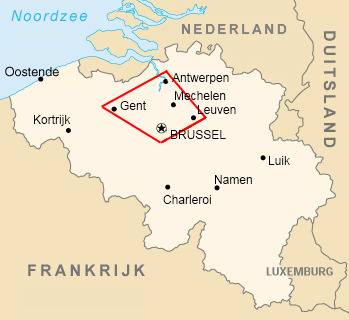
\includegraphics[width=0.99\textwidth]{Vlaamse_ruit}
\end{center}
\end{minipage}
\end{oefening}

\begin{oefening}
De {\em Marginale Driehoek van Vlaanderen} is een denkbeeldige driehoek tussen Diest, Tienen en Aarschot. Naar het schijnt zou Napoleon zijn soldaten uit de lage rangen indertijd naar deze streek gestuurd hebben om uit te rusten in de aanloop naar de Slag van Waterloo.
\begin{enumerate}[(a)]
  \item Bepaal in vogelvlucht de afstanden tussen deze drie steden.
  \item Geef deze afstanden in een matrix weer.
\end{enumerate}
\end{oefening}

\begin{oefening}
De Eurometropool Kortrijk-Rijsel-Doornik is een intercommunale die bedoeling heeft om de samenwerking te verbeteren binnen het grensoverschrijdend grootstedelijk gebied tussen de steden Rijsel, Kortrijk en Doornik.
\begin{enumerate}[(a)]
  \item Bepaal in vogelvlucht de afstanden tussen deze drie steden.
  \item Geef deze afstanden in een matrix weer.
\end{enumerate}
\end{oefening}

\begin{oefening}
Gegeven
$$A=\begin{pmatrix}
  x & y\\
  y & z
\end{pmatrix}$$
Bepaal $x$, $y$ en $z$ als je weet dat $a_{ij}=i+j$.
\end{oefening}

\begin{oefening}
Gegeven
$$A=\begin{pmatrix}
  -4x+3y & -2x+2y\\
  -5x+4y & 5x-2y
\end{pmatrix}$$
Bepaal $x$ en $y$ als je weet dat $a_{ij}=i\cdot j$.
\end{oefening}


\pagebreak
\section{Bijzondere matrices}

\subsection{Nulmatrix}

\paragraph*{Definitie:}

Een {\bf nulmatrix} van orde $m \times n$ is een $m \times n$-matrix waarvan alle elementen gelijk zijn aan nul.

\paragraph*{Notatie:}

$O_{m,n}$

\paragraph*{Voorbeeld:}

$O_{3,2}=
\begin{pmatrix}
  0 & 0 \\ 0 & 0 \\ 0 & 0
\end{pmatrix}
$ is een nulmatrix van orde $3 \times 2$.

\subsection{Rijmatrix}

\paragraph*{Definitie:}

Een {\bf rijmatrix} is een matrix met precies één rij.
\paragraph*{Voorbeeld:}

$A=
\begin{pmatrix}
  1 & 2 & 3
\end{pmatrix}
$ is een rijmatrix.

\subsection{Kolommatrix}

\paragraph*{Definitie:}

Een {\bf kolommatrix} is een matrix met precies één kolom.
\paragraph*{Voorbeeld:}

$B=
\begin{pmatrix}
  4 \\ 5 \\ 6
\end{pmatrix}
$ is een kolommatrix.

\needspace{4cm}
\subsection{Vierkante matrix}

\paragraph*{Definities:}\mbox{}

Een {\bf vierkante matrix} van orde $n$ is een matrix met $n$ rijen en $n$ kolommen. M.a.w. het aantal rijen is gelijk aan het aantal kolommen van een $m \times n$-matrix en dus $m=n$.

De {\bf hoofddiagonaal} van een vierkante $n \times n$-matrix $(a_{ij})_{1 \leq i \leq n , 1 \leq j \leq n}$ is de rij van elementen $a_{11}$, $a_{22}$, \ldots , $a_{nn}$. M.a.w. de rij elementen op de diagonaal die van linksboven schuin naar beneden loopt.

De {\bf nevendiagonaal} van een vierkante $n \times n$-matrix $(a_{ij})_{1 \leq i \leq n , 1 \leq j \leq n}$ is de rij van elementen $a_{n\,1}$, $a_{n-1\,2}$, \ldots , $a_{1\,n}$.

\paragraph*{Voorbeeld:}

De $3 \times 3$-matrix
$$D=
\begin{pmatrix}
  2 & 7 & 6\\
  9 & 5 & 1\\
  4 & 3 & 8\\
\end{pmatrix}
$$
is een vierkante matrix van orde $3$ waarbij de elementen op de hoofddiagonaal
$\begin{pmatrix}2 & 5 & 8\end{pmatrix}$
en de elementen op de nevendiagonaal
$\begin{pmatrix}6 & 5 & 4\end{pmatrix}$
en de elementen in elke rij en de elementen in elke kolom allemaal dezelfde som hebben.

\subsection{Diagonaalmatrix}

\paragraph*{Definitie:}

Een {\bf diagonaalmatrix} is een vierkante matrix waarbij alle elementen die niet op de hoofddiagonaal staan nul zijn

\paragraph*{Voorbeeld:}

$E=
\begin{pmatrix}
  4 & 0 & 0 & 0\\ 0 & 3 & 0 & 0\\ 0 & 0 & 2 & 0\\ 0 & 0 & 0 & 1
\end{pmatrix}
$ is een diagonaalmatrix.

\begin{oefening}
  \begin{enumerate}[(a)]
  \item Is de nulmatrix $O_{22}=\begin{pmatrix}0 & 0\\ 0 & 0\end{pmatrix}$ een diagonaalmatrix?
  \item Is de nulmatrix $O_{23}$ een diagonaalmatrix?
\end{enumerate}
\end{oefening}

\subsection{Scalaire matrix}

\paragraph*{Definitie:}

Een {\bf scalaire matrix} is een diagonaalmatrix $(a_{ij})_{1 \leq i \leq n , 1 \leq j \leq n}$ waarvoor geldt dat $a_{11} = a_{22} = \cdots a_{nn}$. M.a.w. alle elementen op de hoofddiagonaal zijn aan elkaar gelijk.

\paragraph*{Voorbeeld:}

$F=
\begin{pmatrix}
  -5 & 0 \\ 0 & -5
\end{pmatrix}
$ is een scalaire $2 \times 2$-matrix.

\begin{oefening}
  Geef de orde $m \times n$ waarbij een matrix altijd een scalaire matrix zal zijn.
\end{oefening}

\subsection{Driehoeksmatrix}

\paragraph*{Definities:}\mbox{}

Een {\bf bovendriehoeksmatrix} is een vierkante matrix $(a_{ij})_{1 \leq i \leq n , 1 \leq j \leq n}$ waarvoor geldt dat $a_{ij}=0$ met $i > j$. M.a.w. alle elementen onder de hoofddiagonaal zijn nul.

Een {\bf onderdriehoeksmatrix} is een vierkante matrix $(a_{ij})_{1 \leq i \leq n , 1 \leq j \leq n}$ waarvoor geldt dat $a_{ij}=0$ met $i < j$. M.a.w. alle elementen boven de hoofddiagonaal zijn nul.

\paragraph*{Voorbeeld:}

$G=
\begin{pmatrix}
  \dfrac{1}{2} & \dfrac{1}{3} & \dfrac{1}{4} \\
  0            & \dfrac{1}{5} & \dfrac{1}{6} \\
  0            & 0            & \dfrac{1}{7}
\end{pmatrix}
$ is een vierkante matrix en een bovendriehoeksmatrix van de orde $3 \times 3$.


\begin{oefening}
Welke soort matrices zijn zowel boven- als onderdriehoeksmatrices?
\end{oefening}

\subsection{Eenheidsmatrix}

\paragraph*{Definitie:}

Een {\bf eenheidsmatrix} van orde $n$ is een scalaire matrix $(a_{ij})_{1 \leq i \leq n , 1 \leq j \leq n}$ waarvoor geldt dat $a_{ii}=1$. M.a.w. de elementen op de hoofddiagonaal zijn allemaal 1, alle andere elementen zijn 0:

$$
\begin{pmatrix}
  1 & 0 & \cdots & 0 \\
  0 & 1 & \cdots & 0 \\
  \vdots & \vdots & \ddots & \vdots \\
  0 & 0 & \cdots & 1 \\
\end{pmatrix}
$$

\paragraph*{Notatie:} $I_n$ is de eenheidsmatrix van orde $n$.

\paragraph*{Voorbeeld:}

$I_2=
\begin{pmatrix}
  1 & 0 \\ 0 & 1
\end{pmatrix}
$

\subsection{Gelijke matrices}

\paragraph*{Definitie: } We noemen twee matrices $(a_{ij})_{1 \leq i \leq m , 1 \leq j \leq n}$ en $(b_{ij})_{1 \leq i \leq m' , 1 \leq j \leq n'}$ gelijk als $m=m'$ en $n=n'$ en als $a_{ij}=b_{ij}$. M.a.w. als ze beide hetzelfde aantal rijen en kolommen hebben en als elke twee overeenkomstige elementen gelijk zijn.

\paragraph*{Notatie:} $A=B$

\paragraph*{Voorbeeld:}
$
\begin{pmatrix}a^0 & a^1\\ a^2 & a^3\end{pmatrix}
=
\begin{pmatrix}1 & 2\\ 4 & 8\end{pmatrix}
\lra
a = 2$

\needspace{3cm}
\subsection{Oefeningen}

\begin{oefening}
Bepaal $x$ en $y$
%\begin{multicols}{2}
\begin{enumerate}[(a)]
  \item
    $$\begin{pmatrix}
      x & 5\\
      0 & y
    \end{pmatrix}
    =
    \begin{pmatrix}
      1 & 5\\
      0 & 3
    \end{pmatrix}$$
  \item
    $$\begin{pmatrix}
      1 & x\\
      2 & y
    \end{pmatrix}
    =
    -\begin{pmatrix}
      -1 & 4\\
      -2 & -3
    \end{pmatrix}$$
\end{enumerate}
%\end{multicols}
\end{oefening}

\begin{oefening}
Bepaal $x$ en $y$
%\begin{multicols}{2}
\begin{enumerate}[(a)]
  \item
$$\begin{pmatrix}
  x-2y  & 2x+2y\\
  2x-4y & -x+3y
\end{pmatrix}
=
\begin{pmatrix}
  -1 & 10\\
  -2 & 3
\end{pmatrix}$$
  \item
$$\begin{pmatrix}
  4x-6y  & 2x+9y\\
  6x-6y & 4x-6y
\end{pmatrix}
=
\begin{pmatrix}
  0 & 4\\
  1 & 0
\end{pmatrix}$$
  \item
$$\begin{pmatrix}
  3x+4y  & 8x\\
  4x & 5x+y
\end{pmatrix}
=
\begin{pmatrix}
  -14 & -6y\\
  -3y & 22
\end{pmatrix}$$
  \item
$$\begin{pmatrix}
  \sqrt{2}x+\sqrt{3}y  & -\sqrt{2}x+\sqrt{3}y \\
  -\sqrt{2}x-\sqrt{3}y  & \sqrt{2}x-\sqrt{3}y
\end{pmatrix}
=
\begin{pmatrix}
  5 & 1\\
  -5 & -1
\end{pmatrix}$$
\end{enumerate}
%\end{multicols}
\end{oefening}

\begin{oefening}
  Geef van elke matrix de orde. Zeg ook welke bijzonder zijn en tot welke groep ze behoren. Je hebt keuze uit: nulmatrix, rijmatrix, kolommatrix, vierkante matrix, diagonaalmatrix, scalaire matrix, eenheidsmatrix, bovendriehoeksmatrix en/of onderdriehoeksmatrix.\\
  \begin{enumerate}[(a)]
    \itemsep1em
  \item $
    A=\begin{pmatrix}
      -1 & 0\\
      2 & 3\\
      -2 & 1\\
      4 & -3
    \end{pmatrix}
    $
  \item $
    B=\begin{pmatrix}
      -1 & 0 & 0\\
      2 & -1 & 0\\
      -2 & 1 & -1\\
    \end{pmatrix}
    $
  \item $
    C=\begin{pmatrix}
      2 & 0\\
      0 & 2\\
    \end{pmatrix}
    $
  \item $
    D=\begin{pmatrix}
      1
    \end{pmatrix}
    $
  \end{enumerate}
\end{oefening}

\pagebreak
\section{Bewerkingen met matrices}

\subsection{Tegengestelde van een matrix}

\paragraph*{Definitie:} Twee $m \times n$-matrices zijn tegengesteld als hun overeenkomstige elementen elkaars tegengestelde zijn.

\paragraph*{Notatie:} $-A$ is de tegengestelde van $A$

\paragraph*{Opmerking:} De orde wijzigt niet door de tegengestelde te nemen.

\paragraph*{Voorbeeld:} Als
$A=\begin{pmatrix}1 & -2\\ -3 & 4\end{pmatrix}$
dan is
$-A=\begin{pmatrix}-1 & 2\\ 3 & -4\end{pmatrix}$.

\begin{oefening}
  Welke $m \times n$-matrices zijn tegengestelden van zichzelf?
\end{oefening}

\begin{oefening}
  \begin{enumerate}[(a)]
  \item Bepaald de tegengestelde matrix van $\begin{pmatrix}3 & 2\\ 1 & 0\end{pmatrix}$
  \item Bereken \qquad $-\begin{pmatrix}a & -b & 0\\ 0 & c & -d\end{pmatrix}$
  \end{enumerate}
\end{oefening}

\subsection{Optellen van matrices}

\paragraph*{Definitie:} De {\bf som} van twee $m \times n$-matrices $A$ en $B$ is de $m \times n$-matrix die men bekomt door de overeenkomstige elementen bij elkaar op te tellen.

\paragraph*{Notatie:} $A + B$

\paragraph*{Opmerkingen:} De twee matrices kunnen maar opgeteld worden als hun orde gelijk is.

\paragraph*{Voorbeelden:}

\begin{enumerate}[(a)]
\item
  $
  \begin{pmatrix}
    3 & 4 & 5\\
    -2 & 3 & 4\\
    1 & 2 & 3\\
  \end{pmatrix}
  +
  \begin{pmatrix}
    1 & 1 & 2\\
    2 & -4 & 5\\
    2 & 3 & 2
  \end{pmatrix}
  =
  \begin{pmatrix}
    4 & 5 & 7\\
    0 & -1 & 9\\
    3 & 5 & 5
  \end{pmatrix}
  $
\item
  $
  \begin{pmatrix}
    1 & 1\\
    1 & 1\\
    1 & 1
  \end{pmatrix}
  +
  \begin{pmatrix}
    1 & 1\\
    1 & 1\\
    1 & 1
  \end{pmatrix}
  =
    \begin{pmatrix}
    2 & 2\\
    2 & 2\\
    2 & 2
  \end{pmatrix}
  $
\item
  $
  I
  +
  \begin{pmatrix}
    4 & 5\\
    5 & 4
  \end{pmatrix}
  =
  \begin{pmatrix}
    5 & 5\\
    5 & 5
  \end{pmatrix}
  $
\end{enumerate}

\paragraph*{*Eigenschappen:}\mbox{}

\begin{itemize}
\item Het optellen van matrices is {\bf commutatief}:
  $$A+B = B+A$$
\item Het optellen van matrices is {\bf associatief}:
  $$A + (B + C) = (A + B) + C$$
\item De nulmatrix $O_{m,n}$ is het {\bf neutraal element} voor de optelling van $m \times n$-matrices:
  $$A + O_{m,n} = A = O_{m,n} + A$$
\item De tegengestelde matrix $-A$ is het {\bf symmetrisch element} voor de matrix $A$ bij de optelling:
  $$A + (-A) = O_{m,n} = (-A) + A$$
\end{itemize}

\begin{oefening}
  Waarom kunnen we de som van
  $$
  \begin{pmatrix}
    2 & 3 & 4\\
    4 & 3 & 2
  \end{pmatrix}
  \mbox{ en }
  \begin{pmatrix}
    4 & 4\\
    4 & 4
  \end{pmatrix}
  $$
  niet uitrekenen?
\end{oefening}

\subsection{Verschil van twee matrices}

\paragraph*{Definitie:} Het {\bf verschil} van twee $m \times n$-matrices $A$ en $B$ is de som van $A$ met het tegengestelde $-B$.

\paragraph*{Notatie:} $A - B$

We hebben dus dat $A - B = A + (-B)$.

\paragraph*{Voorbeeld:}
$
\begin{pmatrix}
  1 & 2\\
  3 & -4\\
  -5 & -6
\end{pmatrix}
-
\begin{pmatrix}
  -1 & 2\\
  -3 & 4\\
  -5 & 6
\end{pmatrix}
=
\begin{pmatrix}
  2 & 0\\
  3 & -8\\
  0 & -12
\end{pmatrix}
$

\begin{oefening}
  Bereken
  \[
  \begin{pmatrix}
    1 & -3 & -7\\
    9 & -13 & 17
  \end{pmatrix}
  -
  \begin{pmatrix}
    33 & 11 & 17\\
    13 & -13 & 0
  \end{pmatrix}
  \]
\end{oefening}

\begin{oefening}
  Welke matrix kan je van
  $A=
  \begin{pmatrix}
    1 & 2\\ 3 & 4
  \end{pmatrix}
  $
  aftrekken om de nulmatrix $O_{2,2}$ uit te komen?
\end{oefening}

\subsection{Product van een matrix met een reëel getal}

\paragraph*{Definitie:} Het product van een matrix met een reëel getal noemen we een {\bf scalaire vermenigvuldiging} en is de matrix die we bekomen door alle elementen van de gegeven matrix te vermenigvuldigen met dat getal.

We hebben dus als de matrix $A=(a_{ij})_{1 \leq i \leq m , 1 \leq j \leq n}$ wordt vermenigvuldigd met het getal $\lambda$, dan is
$$\lambda \cdot A = \lambda \cdot
\begin{pmatrix}
  a_{11}               & a_{12}               & \cdots & a_{1n}               \\
  a_{21}               & a_{22}               & \cdots & a_{2n}               \\
  \vdots               & \vdots               & \ddots & \vdots               \\
  a_{m1}               & a_{m2}               & \cdots & a_{mn}               \\
\end{pmatrix}
=
\begin{pmatrix}
  \lambda \cdot a_{11} & \lambda \cdot a_{12} & \cdots & \lambda \cdot a_{1n} \\
  \lambda \cdot a_{21} & \lambda \cdot a_{22} & \cdots & \lambda \cdot a_{2n} \\
  \vdots               & \vdots               & \ddots & \vdots               \\
  \lambda \cdot a_{m1} & \lambda \cdot a_{m2} & \cdots & \lambda \cdot a_{mn} \\
\end{pmatrix}
$$

\paragraph*{Voorbeelden:}
\begin{enumerate}[(a)]
\item
  $3 \cdot
  \begin{pmatrix}
    2           & 0 \\
    0.333\ldots & -1
  \end{pmatrix}
  =
  \begin{pmatrix}
    6           & 0 \\
    1           & -3
  \end{pmatrix}
  $
\item
  $\dfrac{1}{2} \cdot
  \begin{pmatrix}
    2           & 4 & 8 & 16
  \end{pmatrix}
  =
  \begin{pmatrix}
    1           & 2 & 4 & 8
  \end{pmatrix}
  $
\end{enumerate}

\begin{oefening}
  Bereken
  $$
  -7 \cdot
  \begin{pmatrix}
    \dfrac{6}{5} & 4.5 & -8\\
    2 & -\dfrac{9}{2} & \dfrac{11}{3}
  \end{pmatrix}
  $$
\end{oefening}

\begin{oefening}
  Welke $\lambda$ moeten we kiezen als we de tegengestelde matrix van $A$ willen bekomen via een scalaire vermenigvuldiging.
\end{oefening}

\paragraph*{*Eigenschappen:}
Als $A,B \in \mathbb{R}^{m \times n}$ en als $\lambda,\,\mu \in \mathbb{R}$, dan geldt
\begin{itemize}
\item $\lambda \cdot (\mu \cdot A) = (\lambda \mu) \cdot A$
\item $\lambda \cdot (A + B) = \lambda \cdot A + \lambda \cdot B$
\item $(\lambda + \mu) \cdot A = \lambda \cdot A + \mu \cdot A$
\item $1 \cdot A = A$
\item $0 \cdot A = O_{m,n}$
\end{itemize}

\subsection{Product van twee matrices}

\paragraph*{Definitie:} Het {\bf product} van een $m \times n$-matrix $A$ met een $n \times p$-matrix $B$ is een $m \times p$-matrix $C$ waarbij het element in de $i$-de rij en $j$-de kolom wordt bekomen door de $i$-de rij van $A$ te {\em vermenigvuldigen} met de $j$-de kolom van $B$. Met dat {\em vermenigvuldigen} bedoelen we dat de elementen van $A$ in de $i$-de rij paarsgewijs vermenigvuldigd worden met de elementen van $B$ in de $j$-de kolom en de bekomen producten worden dan opgeteld.

\paragraph*{Notatie:} $A \cdot B$ of nog korter $AB$

\paragraph*{Voorbeeld:}
\begin{align*}
  \begin{pmatrix}
    1 & 0 & 5\\
    -2 & 3 & -1
  \end{pmatrix}
    \cdot
  \begin{pmatrix}
    0 & 1\\
    2 & 6\\
    4 & -3
  \end{pmatrix}
    &=
  \begin{pmatrix}
    1 \cdot 0 + 0 \cdot 2 + 5 \cdot 4    & 1 \cdot 1 + 0 \cdot 6 + 5 \cdot (-3)\\
    -2 \cdot 0 + 3 \cdot 2 + (-1)\cdot 4 & -2 \cdot 0 + 3 \cdot 6 + (-1) \cdot (-3)
  \end{pmatrix}\\
    &=
  \begin{pmatrix}
    20 & -14\\
    2  & 21
  \end{pmatrix}
\end{align*}

\paragraph*{Opmerking:} We kunnen twee matrices alleen maar met elkaar vermenigvuldigen als het aantal kolommen van de eerste matrix gelijk is aan het aantal rijen van de tweede matrix!
\[
  \begin{pmatrix}
    \vspace{1cm}\hspace{2cm}
  \end{pmatrix}_{m \times \textcolor{gray}{n}}
    \cdot\quad
  \begin{pmatrix}
    \vspace{2cm}\hspace{1cm}
  \end{pmatrix}_{\textcolor{gray}{n} \times p}
    =
  \begin{pmatrix}
    \vspace{1cm}\hspace{1cm}
  \end{pmatrix}_{m \times p}
\]

\begin{oefening}\\
Gegeven:
\[
A=\begin{pmatrix}
  -2 & 7 & 5 & 1\\
  3 & -1 & 0 & -4
\end{pmatrix}_{2 \times 4}
\quad
B=\begin{pmatrix}
  -1\\
  3
\end{pmatrix}_{2 \times 1}
\quad
C=\begin{pmatrix}
  1 & -7\\
  -2 & 0
\end{pmatrix}
\]\[
D=\begin{pmatrix}
  0 & -6\\
  -1 & 0\\
  2 & 4
\end{pmatrix}
\quad
E=\begin{pmatrix}
  0\\
  -3\\
  1\\
  2
\end{pmatrix}
\quad
F=\begin{pmatrix}
  1 & 0 & 0\\
  -3 & 2 & -1\\
  0 & 2 & -2\\
  1 & 4 & 5
\end{pmatrix}
\quad
G=\begin{pmatrix}
  5 & -4\\
  0 & 1\\
  0 & 0\\
  -1 & 7
\end{pmatrix}
\]
Bereken de volgende matrices, indien mogelijk:
\[A \cdot B \qquad A \cdot C \qquad A \cdot D \qquad A \cdot E \qquad A \cdot F \qquad A \cdot G\]
\[B \cdot A \qquad C \cdot A \qquad D \cdot A \qquad E \cdot A \qquad F \cdot A \qquad G \cdot A\]
\[A \cdot A \qquad B \cdot B \qquad C \cdot C \qquad D \cdot D \qquad E \cdot E \qquad F \cdot F\]
\end{oefening}

\paragraph*{Eigenschappen:}
\begin{itemize}
\item Matrices vermenigvuldigen is {\bf associatief}:
  \[A \cdot (B \cdot C) = (A \cdot B) \cdot C\]
\item Een matrix vermenigvuldigen met een nulmatrix maakt een nulmatrix:
  \[A_{m \times n} \cdot O_{n \times p} = O_{m \times p} = O_{m \times n} \cdot B_{n \times p}\]
\item Een matrix vermenigvuldigen met een eenheidsmatrix wijzigt de matrix niet:
  \[A \cdot I = A = I \cdot A\]
\item Matrices vermenigvuldigen is {\em niet} commutatief!
\end{itemize}

\subsection{Getransponeerde van een matrix}

\paragraph*{Definitie:} De {\bf getransponeerde matrix} van een matrix $A$ is de matrix die we bekomen door de rijen te vervangen door de overeenkomstige kolommen.

\paragraph*{Notatie:} $A^T$ \textcolor{gray}{of soms nog ${}^tA$}

\paragraph*{Voorbeelden:}
\begin{itemize}
\item $A=
  \begin{pmatrix}
    1 & 2 & 3\\
    4 & 5 & 6
  \end{pmatrix} \Rightarrow
  A^T=
  \begin{pmatrix}
    1 & 4\\
    2 & 5\\
    3 & 6
  \end{pmatrix}
  $
\item $B=
  \begin{pmatrix}
    a & b & c & d
  \end{pmatrix} \Rightarrow
  B^T=
  \begin{pmatrix}
    a\\
    b\\
    c\\
    d
  \end{pmatrix} \Rightarrow
  \left(B^T\right)^T=
  \begin{pmatrix}
    a & b & c & d
  \end{pmatrix}
  $
\end{itemize}

\paragraph*{Opmerking:} De orde wordt ook gewisseld bij transponeren, dus de getransponeerde van een $m \times n$-matrix is een $n \times m$-matrix.

\paragraph*{Eigenschappen:}
\begin{itemize}
\item $(A^T)^T$
\item $(\lambda \cdot A)^T=\lambda \cdot A^T$
\item $(A + B)^T = A^T + B^T$
\item $(A \cdot B)^T = B^T \cdot A^T$
\end{itemize}

\begin{oefening}
  Bepaal de getransponeerde van
  \begin{multicols}{3}
    \begin{enumerate}[(a)]
    \item $A=
      \begin{pmatrix}
        2 & -5\\
        -5 & 2
      \end{pmatrix}
      $
    \item $B=
      \begin{pmatrix}
        5 & -3\\
        2 & 3
      \end{pmatrix}
      $
    \item $C=
      \begin{pmatrix}
        -5 & 2 & -7\\
        -5 & 2 & -7
      \end{pmatrix}
      $
    \end{enumerate}
  \end{multicols}
\end{oefening}

\needspace{3cm}
\subsection{Oefeningen}

\begin{oefening}\\
Gegeven:
$$
\scriptsize
A=\begin{pmatrix}
  -1 & 0\\
  2 & 3\\
  -2 & 1\\
  4 & -3
\end{pmatrix}
\quad
B=\begin{pmatrix}
  -2 & 3\\
  1 & -4\\
\end{pmatrix}
\quad
C=\begin{pmatrix}
  2 & -1 & 0 & 3\\
  1 & 0 & 4 & -1\\
  -2 & -3 & 1 & 0\\
\end{pmatrix}
\quad
D=\begin{pmatrix}
  -3 & 1 & 0 & 4\\
  2 & -2 & 3 & 1\\
  -1 & 2 & 4 & -3\\
  2 & 0 & -1 & 3\\
\end{pmatrix}
\quad
E=\begin{pmatrix}
  -1\\
  0\\
  2\\
\end{pmatrix}
$$
Bereken:
\begin{multicols}{2}
  \begin{enumerate}[(a)]
    \itemsep1em
    \item $(C\cdot D)^T=$
    \item $(D\cdot C^T\cdot E)^T=$
    \item $2D\cdot A=$
    \item $D^2\cdot C^T=$
    \item $(E^T\cdot C\cdot A)^T=$
    \item $E\cdot D - 2C=$
    \item $B^2\cdot A^T\cdot D=$
    \item $A^T\cdot C^T\cdot E=$
    \item $3B\cdot A^T=$
    \item $E^T\cdot(-C)\cdot 2A=$
  \end{enumerate}
\end{multicols}
\end{oefening}

\begin{oefening}\\
Gegeven:
$$
\scriptsize
A=\begin{pmatrix}
  0 & 3\\
  -2 & -1\\
  2 & 1\\
  3 & -4
\end{pmatrix}
\quad
B=\begin{pmatrix}
  -4 & -3\\
  1 & 0\\
\end{pmatrix}
\quad
C=\begin{pmatrix}
  -2 & 1 & -2 & 0\\
  3 & -1 & -4 & 0\\
  2 & 0 & -1 & -3\\
\end{pmatrix}
\quad
D=\begin{pmatrix}
  1 & -1 & 3 & 0\\
  3 & 2 & 2 & 4\\
  -3 & -4 & 2 & 1\\
  0 & 2 & 1 & -3\\
\end{pmatrix}
\quad
E=\begin{pmatrix}
  0\\
  -2\\
  1\\
\end{pmatrix}
$$
Bereken:
\begin{multicols}{2}
  \begin{enumerate}[(a)]
    \itemsep1em
    \item $(C\cdot D)^T=$
    \item $(D\cdot C^T\cdot E)^T=$
    \item $2D\cdot A=$
    \item $D^2\cdot C^T=$
    \item $(E^T\cdot C\cdot A)^T=$
    \item $E\cdot D - 2C=$
    \item $B^2\cdot A^T\cdot D=$
    \item $A^T\cdot C^T\cdot E=$
    \item $3B\cdot A^T=$
    \item $E^T\cdot(-C)\cdot 2A=$
  \end{enumerate}
\end{multicols}
\end{oefening}

\pagebreak
\section{Migratie- en Lesliematrices}

\begin{oefening}
In een ontwikkelingsland is er een wekelijks mededelingsprogramma voor landbouwers waarin een technologische evolutie wordt uiteengezet. Deze landbouwers hebben onderling geen contact. De kans dat een landbouwer luistert is $20$ \%. We gaan ervan uit dat in het ontwikkelingsland met 250 duizend landbouwers er initieel geen enkele landbouwer iets van de innovaties weet.

\begin{enumerate}[(a)]
  \item Stel de gegevens grafisch voor met behulp van een graaf.
  \item Stel een migratie matrix op.
  \item Hoeveel landbouwers zullen na één maand op de hoogte zijn van de technologische vooruitgang?
  \item Hoeveel landbouwers zullen er na een jaar op de hoogte zijn?
  \item * Dit probleem kan ook opgelost worden m.b.v. {\em exponentiële functies}. Kom op deze oefening terug wanneer je dit in het zesde jaar gezien hebt. Geef een functievoorschrift die het aantal onwetende landbouwers uitdrukt in functie van het aantal maanden dat de radiouitzendingen al spelen. Los dan bovenstaande twee vragen terug op.
\end{enumerate}
\end{oefening}

\begin{oefening}
De migratie tussen de steden Antwerpen, Mechelen en Brussel  voor een periode van 3 jaar
is gegeven door

$$
M = \begin{pmatrix}
  3/5 & 1/10 & 1/10\\
  1/5 & 4/5  & 3/10\\
  1/5 & 1/10 & 3/5
\end{pmatrix}
$$

De bevolking in deze steden is nu Antwerpen – 55, Mechelen – 98, Brussel – 112.

\begin{enumerate}[(a)]
  \item Geef bijhorende graaf.
  \item Geef populatiematrix nu.
  \item Bereken de bevolkingsaantallen na 1, 2 en 3 jaar en voorspel wat er zal gebeuren.
  \item Controleer nu je voorspelling en bereken mbv ICT de bevolkingsaantallen naar een veel jaar.
\end{enumerate}
\end{oefening}

\begin{oefening}% Uit "Enkele didactische wenken voor wiskundeonderwijs in de derde graad" van Koen De Naeghel
Drie telefoonmaatschappijen B, M en P delen de Belgische markt. Maatschappij B heeft 30\% van de markt in handen, M bezit 35\% en P neemt 35\% voor zijn rekening. In de loop van een jaar doen zich de volgende wijzigingen voor:
\begin{itemize}
  \item Maatschappij B behoudt 85\% van de klanten, terwijl het 10\% aan M en 5\% aan P verliest.
  \item Maatschappij M behoudt 55\% van de klanten, terwijl het 20\% aan B en 25\% aan P verliest.
  \item Maatschappij P behoudt 85\% van de klanten, terwijl het 10\% aan M en 5\% aan B verliest.
\end{itemize}
We nemen aan dat deze wijziging zich elk jaar opnieuw voordoet.

\begin{enumerate}[(a)]
  \item Stel de evolutie van de markt voor met een graaf.
  \item Stel een migratie matrix op.
  \item Hoe evolueert de Belgische markt?
\end{enumerate}
\end{oefening}

\begin{oefening}
Eva en Kasper, twee ornithologen, hebben een nieuwe vogelsoort ontdekt in het tropische Amazonegebied.  Het gaat over een kleine vogelsoort die heel wat weg heeft van een kolibrie.  Na jaren observatie komen ze tot de volgende conclusies :
\begin{itemize}
  \item slechts 30\% van de eieren komt uit en bereikt de leeftijd van één jaar
  \item de kans om het volgende levensjaar te halen is steeds 70\%
  \item geen enkele vogel wordt ouder dan vijf jaar
  \item elke 2-jarige en 3-jarige vogel legt gemiddeld twee eieren,
  \item elke 4-jarige vogel gemiddeld slechts één ei
\end{itemize}
Men telde in het broedseizoen (in mei dus) van 2016 de volgende populatie :
80 éénjarigen, 50 tweejarigen, 30 driejarigen, 20 vierjarigen en 180 eieren (of nuljarigen).

\begin{enumerate}[(a)]
  \item Stel de gegevens grafisch voor.
  \item Geef de corresponderende lesliematrix en populatiematrix voor 2016.
  \item Geef de populatie in 2017 en in 2018.
\end{enumerate}
\end{oefening}

\begin{oefening}
Veronderstel dat we een bepaalde vissoort hebben die enkel tijdens het derde levensjaar reproduceert en dan sterft. Veronderstel dat we initieel 1000 jonge visjes hebben van deze soort en geen andere vissen. Veronderstel dat 25\% van de eenjarigen overleeft en dat dan 50\% van de visjes het maken tot de vruchtbare leeftijd.
\begin{enumerate}[(a)]
  \item Onderzoek hoe de populatie evolueert als het reproductiecijfer 8 is, m.a.w. als een vruchtbaar visje 8 nakomelingen heeft.
  \item Doe nu hetzelfde onderzoek, maar dan met een hoger en/of lager reproductiecijfer. {\em Het is toegelaten om verbaast te zijn!}
\end{enumerate}
\end{oefening}

\pagebreak
\section{Gauss-Jordan}

\begin{oefening}
Los op in $\mathbb{R}^3$:
\begin{multicols}{2}
\begin{enumerate}[(a)]
  \item$$\left\{
\begin{aligned}
  x + 2y -z &= -4\\
  2x+3y+z   &= 3\\
  5x-y+3z   &= 1
\end{aligned}\right.$$
  \item$$\left\{
\begin{aligned}
  -3x -7y +6z &= 6\\
  x+3y-2z   &= 0\\
  2x+y+4z   &= 25
\end{aligned}\right.$$
  \item$$\left\{
\begin{aligned}
  3x +2y +4z &= -4\\
  x+y+z   &= 1\\
  5x-4y+3z   &= -3
\end{aligned}\right.$$
  \item$$\left\{
\begin{aligned}
  3x -4y +z &= 35\\
  x-y+2z   &= 11\\
  -5x+2y-2z   &= -26
\end{aligned}\right.$$
  \item$$\left\{
\begin{aligned}
  x -y + 2z &= -1\\
  4x-3y+5z   &= 18\\
  -x+y+4z   &= -5
\end{aligned}\right.$$
\end{enumerate}
\end{multicols}
\end{oefening}

\begin{oefening}
Los op in $\mathbb{R}^3$:
\begin{multicols}{2}
\begin{enumerate}[(a)]
  \item$$\left\{
    \begin{aligned}
      3x - 7y + 2z &= 2\\
      -x + 3y      &= -2\\
      x  - 2y +  z &= 0
    \end{aligned}\right.$$
  \item$$\left\{
    \begin{aligned}
        x - 3y -  z &= 2\\
      -2x + 5y + 3z &= 4\\
       4x -11y - 5z &= 5
    \end{aligned}\right.$$
  \item$$\left\{
    \begin{aligned}
      2x + 3y + 5z &= 9\\
       x + 2y + 3z &= 4\\
       x +  z &= 5
    \end{aligned}\right.$$
  \item$$\left\{
    \begin{aligned}
      2x +  y - 2z &= -2\\
      3x + 2y -  z &=  4\\
       x +  y +  z &=  6
    \end{aligned}\right.$$
  \item$$\left\{
    \begin{aligned}
       x + 2y +  z &= 3\\
      2x + 3y + 4z &= 5\\
      4x + 7y + 6z &= 9
    \end{aligned}\right.$$
\end{enumerate}
\end{multicols}
\end{oefening}

\begin{oefening}
Los op in $\mathbb{R}^3$:
\begin{multicols}{2}
\begin{enumerate}[(a)]
  \item$$\left\{
    \begin{aligned}
      3x -  y +  z &= 29\\
      x  + 3y +30z &=  6\\
      x  -  y +  z &= 17
    \end{aligned}\right.$$
  \item$$\left\{
    \begin{aligned}
      -2x + 4y - 6z &= -46\\
       3x +  y + 38 &= 4z\\
      -4x - 5y + 2z &= 56
    \end{aligned}\right.$$
  \item$$\left\{
    \begin{aligned}
       y - 3x - 2z &= -17\\
      4x +  z - 3y &= 31\\
      2y +  x &= -13 + 4z
    \end{aligned}\right.$$
  \item$$\left\{
    \begin{aligned}
      7z + 3x + 14 &= y\\
       y -  x - 3z &= 4\\
       z - 5x - 3y &= 4
    \end{aligned}\right.$$
  \item$$\left\{
    \begin{aligned}
      2x -  y + 3z &= -4\\
       x + 5z      &= 7\\
      2y +  z + 3x &= 1
    \end{aligned}\right.$$
\end{enumerate}
\end{multicols}
\end{oefening}

\pagebreak
\section{Vraagstukken op stelsels}

\begin{oefening}
In een winkeltje in het dorp kost 200 gram nougat, 300 gram chocolaatjes en 100 gram marsepein
9 EUR.  Voor 300 gram nougat, 100 gram chocolaatjes en 400 gram marsepein betaal je 12,7 EUR.
Hoeveel kost 200 gram nougat, 200 gram chocolaatjes en 200 gram marsepein als je weet dat
1 kg chocolaatjes 5 euro minder kost dan 1 kg nougat?
\end{oefening}

\begin{oefening}
Boer Moors kweekt geiten, schapen en struisvogels.  Toen ik hem vroeg hoeveel stuks hij van elke soort had, kreeg ik het volgende antwoord.\\
“Wanneer één derde van mijn geiten schapen zou zijn, had ik evenveel geiten als schapen en struisvogels samen.
Wanneer één derde van mijn schapen struisvogels zou zijn, had ik vijfmaal zoveel geiten als struisvogels.
Wanneer één derde van mijn struisvogels geiten zou zijn, had ik 470 geiten.”\\
Kan jij achterhalen hoeveel geiten, schapen en struisvogels boer Moors heeft?
\end{oefening}

\begin{oefening}
“Hoe oud ben je?” vraagt een jongen aan een meisje.
“Wel”, zegt ze, “mijn mama en ik zijn samen 56 jaar.  Mijn oma en ik zijn samen 80 jaar en mijn mama en mijn oma zijn samen 100 jaar.”
Hoe oud zijn het meisje, haar mama en haar oma?
\end{oefening}

\begin{oefening}
Anke, Bert en Chris willen een geschenk kopen voor het huwelijk van een vriend en vriendin.
Ze overlopen samen hoeveel geld ze hebben.
Anke en Bert hebben samen 20 euro meer dan Chris.
Bert en Chris hebben samen 32 euro meer dan Anke.
Anke en Chris hebben samen 28 euro meer dan Bert.
Hoeveel heeft ieder nog in zijn portemonnee?
\end{oefening}

\begin{oefening}
Anna, Brigitte en Charlotte vormen een driegeslacht.  Samen zijn ze 105 jaar oud.  Anna is negen jaar ouder dan Brigitte en Charlotte samen.  Jammer genoeg komen Anna en Charlotte samen nog drie jaartjes tekort om dubbel zo oud te zijn als Brigitte.
Hoe oud zijn deze drie dames?
\end{oefening}

\begin{oefening}
Bepaal de vergelijking $y=ax^2+bx+c$ van de parabool die door de punten $(1,1)$, $(-1, 5)$ en $(2,2)$ gaat.
\end{oefening}

\begin{oefening}
Bepaal een natuurlijk getal bestaande uit drie cijfers. Het cijfer van de tientallen is het gemiddelde van het cijfer van de honderdtallen en het cijfer van de eenheden. Telt men 396 op bij het getal, dan bekomt men een getal met dezelfde cijfers als het gevraagde getal maar in omgekeerde volgorde. Deelt men het getal door de som van de cijfers, dan is het quotiënt 26 en de rest 0.
\end{oefening}

\begin{oefening}
Een melkveehoudersbedrijf wenst een aantal tankwagens te kopen om zelf de melk te transporteren. Ze kunnen 24 tankwagens kopen en in het totaal moeten ze daarmee 250000 liter melk vervoeren. Er zijn drie types tankwagens aanwezig, tankwagens met een inhoud van 6000, van 8000 en van 18000 liter. Hoeveel tankwagens van elk type zijn nodig.
\end{oefening}

\begin{oefening}
Bepaal het functievoorschrift van een veeltermfunctie $f$ van de derde graad waarvoor $-1$ en $2$ nulwaarden zijn en waarvoor geldt:
$$f(1)=f(-2)=-4$$
\end{oefening}

\begin{oefening}
Bepaal het functievoorschrift van een monische derdegraadsfunctie $f$ die als nulwaarde $1$ en $2$ heeft en waarvoor $(5,120)\in f$ is.
\end{oefening}

\begin{oefening}
Een cirkel gaat door de punten $(2,-2)$, $(-1, -3)$ en $(-2,8)$. Geef de vergelijking van de cirkel.
\end{oefening}

\begin{oefening}
Een diëtist in een ziekenhuis moet een speciaal dieet samenstellen bestaande uit drie ingrediënten. Het dieet moet juist 340 eenheden calcium, 180 eenheden ijzer en 220 eenheden vitamine A bevatten. Het aantal eenheden per $30$ gram van de drie ingrediënten wordt gegeven door de volgende tabel:
\begin{center}
  \begin{tabular}{lccc}
               &\multicolumn{3}{c}{Eenheden per 30 gram}\\
    \hline
               & ingrediënt A & ingrediënt B & ingrediënt C\\
    \hline
    Calcium    & 30           & 10           & 20\\
    Iron       & 10           & 10           & 20\\
    Vitamine A & 10           & 30           & 20\\
  \end{tabular}
\end{center}
\begin{enumerate}[(a)]
  \item Hoeveel gram van elk ingrediënt moet gebruikt worden om te voldoen aan het dieet?
  \item Hoe wordt het dieet beïnvloed als we ingrediënt C niet mogen gebruiken?
  \item Hoe wordt het dieet beïnvloed als we niet langer moeten voldoen aan de vitamine A vereiste?
\end{enumerate}
\end{oefening}

\end{document}
